\documentclass[11pt,a4paper]{article}
\usepackage{tikz}
\usetikzlibrary{arrows.meta,positioning}
\usepackage{tabularx}
\usepackage{amsmath,amssymb,amsthm}
\usepackage{geometry}
\geometry{margin=1in}
\usepackage{hyperref}
\usepackage{graphicx}
\usepackage{setspace}
\onehalfspacing

\title{\textbf{Paper A-06: Ecological Energy and Trophic Networks:\\ A Constraint-Driven Flux Dynamics (CDFD) Perspective}}
\author{Steve Bico Mujjabi, MD\\
\small Independent Researcher\\
\small Founder, Vura Labs\\
\small Kampala, Uganda\\
\small ORCID: 0009-0001-0556-5516}
\date{August 2026}

\begin{document}
\maketitle

% BEGIN SHARED-METHODS POINTER
\noindent\textit{Shared Part IV notation and evidence boundaries are defined in \path{PART_IV_METHODS_AND_CLAIM_BOUNDARY.md}. This paper states only its local observables, comparison, and failure conditions.}
% END SHARED-METHODS POINTER


\begin{abstract}
This paper develops a falsifiable CDFD/AFL model of Earth Ecological Energy Transport. It maps solar energy, nutrients, biomass production, and consumer demand to driving flux $\Phi$, stoichiometry, trophic bottlenecks, habitat limits, and loss to active constraint $C$, functional diversity, migration, storage, and trophic rerouting to responsiveness $S$, and community composition, soil state, disturbance, and evolutionary legacy to structural memory $M_s$. The target outcome is productivity, respiration, transfer efficiency, and recovery, tested against flux towers, food-web observations, isotope tracers, productivity, and respiration records. The paper treats universality as a shared model architecture rather than an assertion that unlike systems have the same material mechanism. It states the negative result that would make the mapping unnecessary and places the domain claim inside the cumulative CDFD programme and its reproducible runtime boundary.
\end{abstract}
% BEGIN CONSOLIDATION SCOPE
\section*{Consolidation Scope and Provenance}
This consolidated paper retains the ecological energy-transport and trophic-network scopes formerly carried by Papers A-06 and D-08. It distinguishes ecosystem productivity and transfer efficiency from trophic-cascade outcomes, and requires field-native ecological baselines for either task.
% END CONSOLIDATION SCOPE


\section{Introduction}

An ecosystem is a biological engine. It captures high-grade solar energy via photosynthesis and dissipates it as heat, passing the intermediate chemical energy up through successive trophic levels. The efficiency of this energy transfer is notoriously low (the 10\% rule), meaning the higher trophic levels are inherently fragile, operating at the absolute limit of available flux.

In CDFD, the food web is not a static list of species; it is a highly active, constraint-bound transport network. Extinction and population booms are simply the system's attempt to regulate its internal fluid pressure.

\section{The Ecological Adaptive Surface}
We govern the trophic network using the Adaptive Operating Ratio:
\begin{equation}
    \Psi_s = \left( \frac{\Phi}{C} \right) \cdot S \cdot M_s
\end{equation}

For an ecosystem (e.g., a coral reef or a savannah):
\begin{itemize}
    \item \textbf{Flux ($\Phi$)}: The caloric energy transfer (biomass consumed) moving from prey to predator.
    \item \textbf{Constraint ($C$)}: The carrying capacity of the environment, including resource scarcity, habitat boundaries, and metabolic friction (heat loss).
    \item \textbf{Responsiveness ($S$)}: The biodiversity and phenotypic plasticity of the ecosystem. A highly diverse ecosystem can quickly reroute energy flow if one specific prey species declines.
    \item \textbf{Memory ($M_s$)}: Niche specialization and symbiotic dependencies. Over millions of years, species become hyper-specialized (high memory). While highly efficient in stable environments, this locks the topological routing of energy into rigid, fragile pathways.
\end{itemize}

\subsection{Trophic Cascades and Keystone Species}
A stable ecosystem balances at $\Psi_s \approx 1$. The caloric flux $\Phi$ perfectly supports the existing constraints and biomass.

Consider the removal of a keystone species (e.g., apex predators like wolves). Without the downward predatory constraint, the herbivore population (flux $\Phi$) explodes. The system enters an over-flux regime ($\Psi_s \gg 1$). The herbivores rapidly consume all available primary producers, completely destroying the foundational responsiveness ($S$) of the environment. The adaptive ratio then crashes violently to $\Psi_s \ll 1$, resulting in a mass die-off.

Conversely, consider an ecosystem locked by high memory $M_s$ (hyper-specialization, like Pandas relying solely on bamboo). If the bamboo is wiped out, the specific energy flux $\Phi$ drops to zero. Because the system's memory is locked, it cannot adapt to a new food source (cannot adjust $C$ or $S$). The isolated node faces immediate necrosis (extinction).



\section{Measurement Layer}

% BEGIN PART IV MAJOR CROSS-DOMAIN UPGRADE
\section{Cross-Domain Model Upgrade: Mechanism, Scale, and Tests}

\subsection{Observable Translation}

The paper-specific translation begins with an observable chain rather than a
verbal analogy. For Earth Ecological Energy Transport, the proposed drive is solar energy, nutrients, biomass production, and consumer demand.
The active limitation is stoichiometry, trophic bottlenecks, habitat limits, and loss. Responsiveness is carried by
functional diversity, migration, storage, and trophic rerouting, while retained state is represented by
community composition, soil state, disturbance, and evolutionary legacy. The outcome to explain is productivity, respiration, transfer efficiency, and recovery.

\begin{table}[htbp]
\centering
\small
\caption{Operational CDFD/AFL map for Paper A-06.}
\begin{tabularx}{\textwidth}{|l|X|X|}
\hline
\textbf{Term} & \textbf{Paper-specific observable meaning} & \textbf{Measurement question} \\
\hline
$\Phi$ & solar energy, nutrients, biomass production, and consumer demand & What rate, load, gradient, or demand enters the focal system? \\
\hline
$C$ & stoichiometry, trophic bottlenecks, habitat limits, and loss & Which measured bottleneck limits transfer, function, or recovery? \\
\hline
$S$ & functional diversity, migration, storage, and trophic rerouting & Which process changes effective capacity or reroutes the load? \\
\hline
$M_s$ & community composition, soil state, disturbance, and evolutionary legacy & Which retained state makes equal present loads produce different futures? \\
\hline
$Y$ & productivity, respiration, transfer efficiency, and recovery & Which outcome is predicted out of sample, with uncertainty? \\
\hline
\end{tabularx}
\end{table}

\begin{figure}[htbp]
\centering
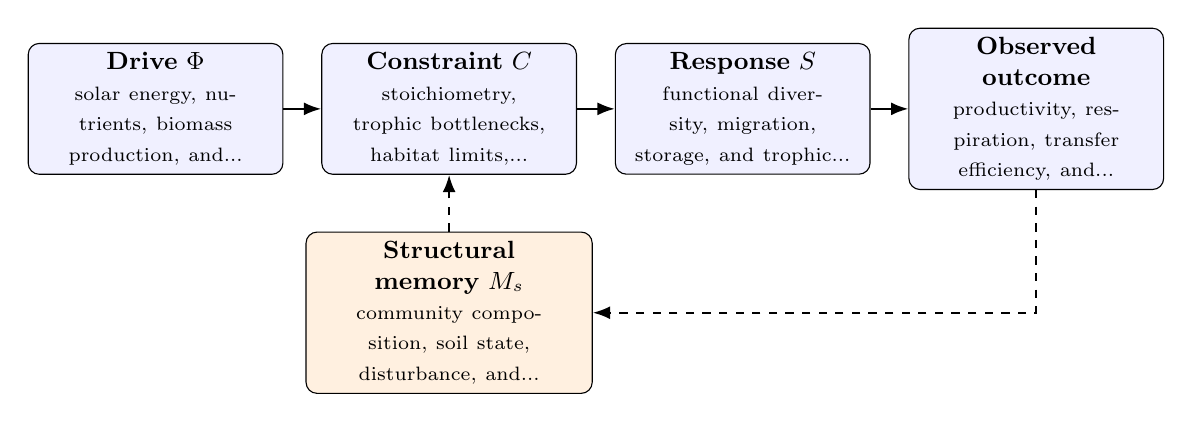
\begin{tikzpicture}[
    node distance=0.48cm,
    every node/.style={font=\small},
    box/.style={draw, rounded corners, align=center, minimum height=1.45cm, text width=3.0cm, fill=blue!6},
    memory/.style={draw, rounded corners, align=center, minimum height=1.25cm, text width=3.4cm, fill=orange!12},
    flow/.style={-{Latex[length=2.2mm]}, thick},
    feedback/.style={-{Latex[length=2.2mm]}, thick, dashed}
]
\node[box] (drive) {\textbf{Drive $\Phi$}\\\scriptsize solar energy, nutrients, biomass production, and...};
\node[box, right=of drive] (constraint) {\textbf{Constraint $C$}\\\scriptsize stoichiometry, trophic bottlenecks, habitat limits,...};
\node[box, right=of constraint] (response) {\textbf{Response $S$}\\\scriptsize functional diversity, migration, storage, and trophic...};
\node[box, right=of response] (outcome) {\textbf{Observed outcome}\\\scriptsize productivity, respiration, transfer efficiency, and...};
\node[memory, below=0.72cm of constraint] (memory) {\textbf{Structural memory $M_s$}\\\scriptsize community composition, soil state, disturbance, and...};
\draw[flow] (drive) -- (constraint);
\draw[flow] (constraint) -- (response);
\draw[flow] (response) -- (outcome);
\draw[feedback] (outcome.south) |- (memory.east);
\draw[feedback] (memory.north) -- (constraint.south);
\end{tikzpicture}
\caption{Paper A-06 observable CDFD/AFL architecture for Earth Ecological Energy Transport. Solid arrows give the proposed forward chain; dashed arrows make history-dependent feedback explicit.}
\label{fig:a06-architecture}
\end{figure}

\subsection{Paper-Specific Causal Hypothesis}

For this paper, the hypothesized causal sequence is specific. A change in
solar energy, nutrients, biomass production, and consumer demand arrives faster than functional diversity, migration, storage, and trophic rerouting can compensate.
This raises or redistributes stoichiometry, trophic bottlenecks, habitat limits, and loss. If the load persists,
the retained state encoded by community composition, soil state, disturbance, and evolutionary legacy changes the next response, so a later event of equal
magnitude can produce a different trajectory in productivity, respiration, transfer efficiency, and recovery. The
scientific task is to estimate that sequence against the best ordinary model of
the domain, not merely to redescribe the outcome after it occurs.

\subsection{Cross-Scale Translation Without Mechanistic Erasure}

For the Earth systems family, the cross-domain translation compares coupled transport, finite environmental capacity, buffering, and retained landscape or ecosystem state. It cannot erase conservation laws, geometry, or scale; it must expose where those domain equations create comparable overload and recovery structures. \cite{Holling1973,Turing1952,BakTangWiesenfeld1987}
The required scale declaration for this paper is seconds to centuries; organisms to biomes. At short
scales, the key question is whether the incoming drive is transmitted,
buffered, or diverted. At intermediate scales, response changes effective
capacity and network exposure. At long scales, retained structure can alter the
state space itself. A result is genuinely cross-scale only when the aggregation
rule is stated and the same conclusion is not an artifact of averaging.

\subsection{Evidence Ladder and Discriminating Tests}

\begin{table}[htbp]
\centering
\small
\caption{Evidence ladder for Paper A-06. Each rung can fail independently.}
\begin{tabularx}{\textwidth}{|p{0.17\textwidth}|X|X|}
\hline
\textbf{Test} & \textbf{Design} & \textbf{Discriminating result} \\
\hline
Proxy audit & Measure flux towers, food-web observations, isotope tracers, productivity, and respiration records and preregister how each record maps to $\Phi$, $C$, $S$, $M_s$, and $Y$. & The mapping fails if proxies are non-identifiable, circular, or change meaning across cases. \\
\hline
Load ramp & Apply or observe a resource pulse followed by drought, harvest, or consumer loss while estimating the dominant constraint and response time. & A threshold claim requires a reproducible nonlinear change and uncertainty bounds, not a visually chosen breakpoint. \\
\hline
Recovery and memory & Match present load across units with different histories, then compare recovery paths. & The memory claim requires history-dependent divergence after current conditions are controlled. \\
\hline
Model comparison & Compare the baseline domain model with and without the CDFD/AFL state variables using held-out data. & The paper's stated falsifier is: the proposed constraint-memory terms do not explain transfer efficiency or recovery. \\
\hline
\end{tabularx}
\end{table}

\subsection{Research Programme and Boundary Conditions}

The immediate research programme has four steps. First, construct a documented
dataset from flux towers, food-web observations, isotope tracers, productivity, and respiration records and retain raw units before normalization.
Second, fit a baseline domain model and report its calibration and out-of-sample
error. Third, add the smallest identifiable CDFD/AFL state extension and test
whether it improves prediction of productivity, respiration, transfer efficiency, and recovery. Fourth, repeat the
analysis across the declared scale range and publish negative cases as part of
the cross-domain translation audit.

% END PART IV MAJOR CROSS-DOMAIN UPGRADE

\section{Conclusion}
Ecosystems are macroscopic thermodynamic circuits. Biodiversity is not merely an aesthetic preference; it is the critical Responsiveness ($S$) parameter that prevents topological gridlock. By applying CDFD, conservation biology gains a unified physics framework: preserving nature requires maintaining the mathematical elasticity of its energy transport networks.
\section*{Conflict of Interest} The author declares no conflict of interest.
\section*{Data Availability}
Part-specific runtime diagnostics are under each Part's \path{outputs/} directory.

Release-wide code: \path{Part_E_Synthesis/supplementary/}.

Generated summaries: \path{Part_E_Synthesis/outputs/}.

Figures: \path{Part_E_Synthesis/figures/}.


\section{Reference Layer}
\bibliographystyle{plain}
\bibliography{universal_afl_references}
\end{document}
